\section{Network Workbench Tool}

% 
\includegraphics[width=90mm]{nwb-graphics/nwbLogo.jpg}

The Network Workbench (NWB) Tool \cite{nwb} is a large-scale network analysis, 
modeling, and visualization toolkit for biomedical, social science, and physics 
research (see page 1). The NWB Tool rebrands the CIShell Reference GUI and 
provides a custom filling of datasets, algorithms, and converters relevant for 
the network science community.
%\\
%\\
%\noindent
%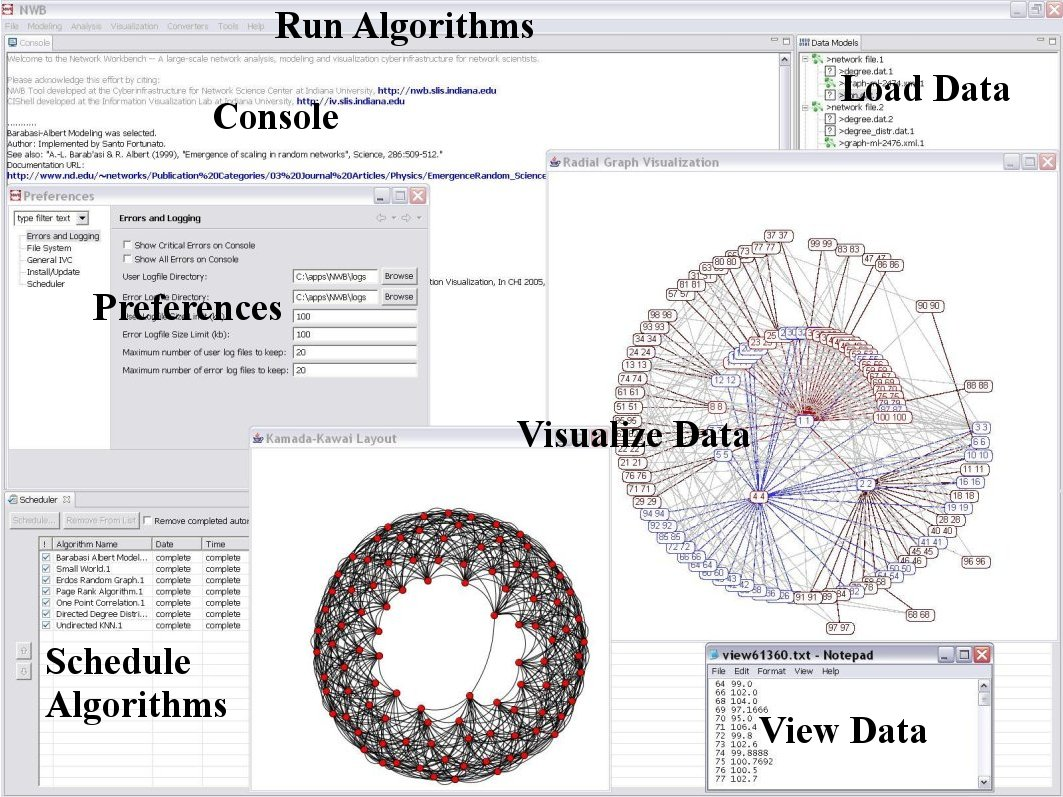
\includegraphics[width=90mm]{nwb-graphics/nwbScreenshot.jpg}

The NWB Tool uses the CIShell data conversion service and a set of converters 
to support the loading and saving of GraphML (.xml), XGMML (.xml), Pajek (.net), 
and Network Workbench (.nwb) formatted files.

%\subsection{Integrated Algorithms \& Datasets}
The current version of the NWB Tool gives easy access to 41 algorithms and a 
few sample datasets. About half of the algorithms were implemented in FORTRAN 
and integrated by a physicist using CIShell's static executable algorithm 
integration template. A listing of the currently integrated algorithms follows.

\begin{multicols}{2}{
\noindent
\begin{tiny} 
\textbf{Sampling}
\begin{list}{}{\setlength{\itemindent}{-7mm}\setlength{\itemsep}{0mm}\setlength{\topsep}{1mm}}
\item Directory Hierarchy Reader
\end{list}
\textbf{ Analysis}
\begin{list}{}{\setlength{\itemindent}{-7mm}\setlength{\itemsep}{0mm}\setlength{\topsep}{1mm}}
\item Node Degree
\item Node Indegree
\item Node Outdegree
\item Undirected Degree Distribution
\item Indegree Distribution
\item Outdegree Distribution
\item Undirected k-Nearest Neighbor
\item Directed k-Nearest Neighbor
\item One Point Correlations
\item Watts Strogatz Clustering Coefficient
\item Watts Strogatz Clustering Coefficient Over k
\item Average Path Length
\item Diameter
\item Distribution of shortest path length
\item Betweenness Centrality
\item Number of Connected Components
\item Page Rank
\item Attack Tolerance
\item Error Tolerance
\item k Random-Walk Search
\item Random Breadth First Search
\item CAN Search
\item Chord Search
\end{list}
\textbf{Modeling}
\begin{list}{}{\setlength{\itemindent}{-7mm}\setlength{\itemsep}{0mm}\setlength{\topsep}{1mm}}
\item Barab\'{a}si-Albert Scale-Free Model
\item CAN Model
\item Chord Model
\item Hypergrid Model
\item PRU Model
\item Erdos-R\'{e}nyi Random Graph Model
\item Watts-Strogatz Small World Model
\end{list}
\textbf{Visualization}
\begin{list}{}{\setlength{\itemindent}{-7mm}\setlength{\itemsep}{0mm}\setlength{\topsep}{1mm}}
\item Circular Layout
\item Radial Tree
\item Tree Map
\item Tree Visualization
\item Force Directed
\item Spring Layout
\item Kamada-Kawai
\item Fruchterman-Reingold
\item Parallel Coordinates (demo)
\end{list}
\textbf{Tool}
\begin{list}{}{\setlength{\itemindent}{-7mm}\setlength{\itemsep}{0mm}\setlength{\topsep}{1mm}}
\item XMGrace
\item 
\item 
\end{list}
\end{tiny}
}
\end{multicols}

%\subsection{Supported File Formats}


\section{NWB Community Wiki}

The Network Workbench Community Wiki \cite{nwbCommunityWiki} is a place for 
users of the Network Workbench Tool, the Cyberinfrastructure Shell, or any 
other CIShell-based application to upload, download, and request datasets and
algorithms. The site (see figure below) was created so that the network science 
community can collaboratively create a tool which meets their needs and the 
needs of the scientific community at large. Users can post want-ads for 
algorithms and datasets to be integrated into CIShell/NWB, and learn how to use 
the resources for their own research.

\begin{center}
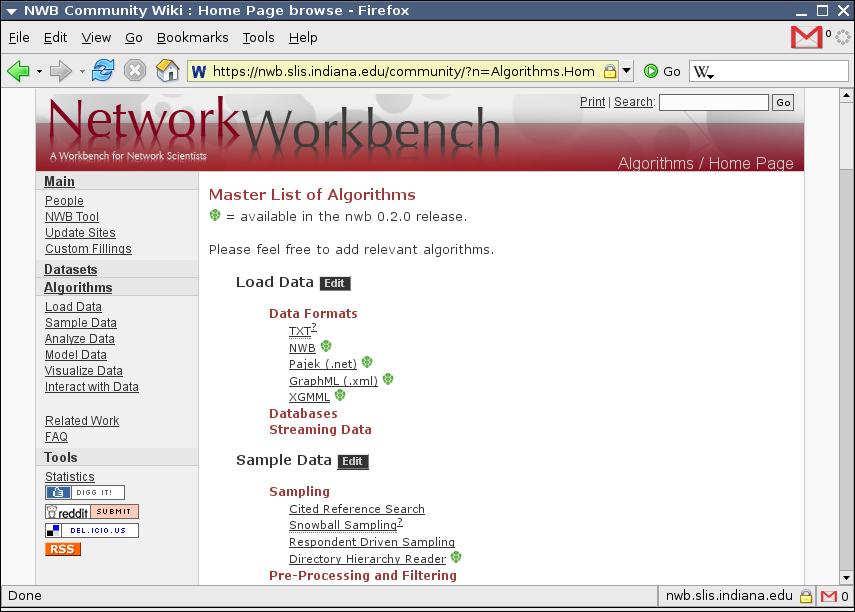
\includegraphics[width=2.85in]{nwb-graphics/nwbWiki.png}
\end{center}